\newpage
\section{Diskussion}
\subsection{Aussagekraft}
In dem Diagramm \ref{fig:} und \ref{fig:} wird deutlich, dass die
Theoriekurve eine diskrepanz gegenüber der aus den Messdaten approximierten 
Kurve bildet, wenn gleich die Kurven ähnlich verlaufen.\\
Der Ursprung dieser Diskrepanz könnte dabei auf einen systematischen Fehler
bei der Kraftmessung zurückgeführt werden. Dennoch liegt näher dass die Differenz
aufgrund der Drahtdicke auftritt, da as Material großen Schwangungen unterlegen ist 
und somit von dem, in der Zeichnung angegeben Wert $d=0.430\si{mm}$ abweicht.\\
Für einen deckungsgleichen Verlauf der beiden Kurven folgt aus Gl. \ref{eqn:federrate} für die Drahtdicke $d$,
\begin{align*}
    R(d)&=\frac{D}{8} \cdot \frac{d^4}{(D_a-d)^3\cdot \frac{L0-LH}{d}},\\
    0&\overset{\text{!}}{=}\frac{D}{8} \cdot \frac{d^4}{(D_a-d)^3\cdot \frac{L0-LH}{d}}-R,
\end{align*}
mit der real Drahtdicke $d_{real}=$  

\begin{figure}
    \center
    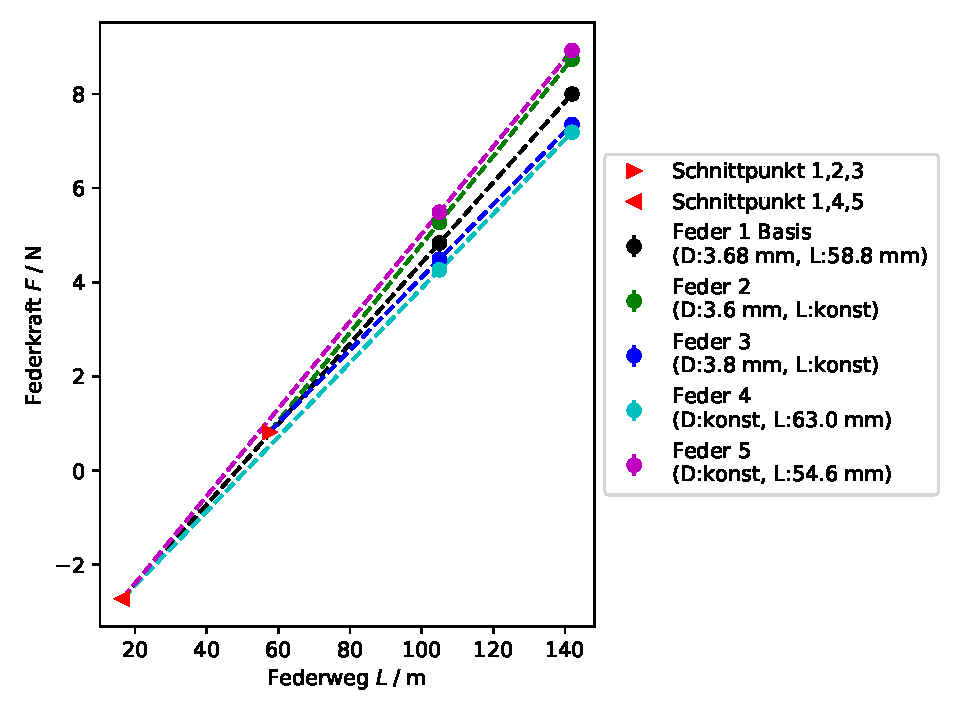
\includegraphics[width=0.8\textwidth]{plots/diss_kraft_dia.pdf}
    \caption{
        Vergleich der Wirkung der veränderlichen Windungszahl $n$ und
        des Federaußendruchmesser $D_a$ auf die Federkraft $F$ untereinander.
    }
\end{figure}

\subsection{Vergleich}

\begin{figure}[H]
    \center
    \includegraphics[width=0.8\textwidth]{plots/schnö_12_dia.pdf}
    \caption{}
\end{figure}

\label{sec:Diskussion}
